% --------------------------------------------------------------
% This is all preamble stuff that you don't have to worry about.
% Head down to where it says "Start here"
% --------------------------------------------------------------

\documentclass[12pt]{article}

\usepackage[margin=1in]{geometry}
\usepackage{amsmath,amsthm,amssymb}
\usepackage{tikz}

\newcommand{\N}{\mathbb{N}}
\newcommand{\Z}{\mathbb{Z}}

\newenvironment{theorem}[2][Theorem]{\begin{trivlist}
\item[\hskip \labelsep {\bfseries #1}\hskip \labelsep {\bfseries #2.}]}{\end{trivlist}}
\newenvironment{lemma}[2][Lemma]{\begin{trivlist}
\item[\hskip \labelsep {\bfseries #1}\hskip \labelsep {\bfseries #2.}]}{\end{trivlist}}
\newenvironment{exercise}[2][Exercise]{\begin{trivlist}
\item[\hskip \labelsep {\bfseries #1}\hskip \labelsep {\bfseries #2.}]}{\end{trivlist}}
\newenvironment{question}[2][Question]{\begin{trivlist}
\item[\hskip \labelsep {\bfseries #1}\hskip \labelsep {\bfseries #2.}]}{\end{trivlist}}
\newenvironment{proposition}[2][Proposition]{\begin{trivlist}
\item[\hskip \labelsep {\bfseries #1}\hskip \labelsep {\bfseries #2.}]}{\end{trivlist}}
\newenvironment{corollary}[2][Corollary]{\begin{trivlist}
\item[\hskip \labelsep {\bfseries #1}\hskip \labelsep {\bfseries #2.}]}{\end{trivlist}}

\begin{document}

% --------------------------------------------------------------
%                         Start here
% --------------------------------------------------------------

%\renewcommand{\qedsymbol}{\filledbox}

\title{Homework 2}%replace X with the appropriate number
\author{Team F\\ %replace with your name
CSC 565 - Graph Theory} %if necessary, replace with your course title

\maketitle

\begin{question}{1}
Find a graph G with 5 vertices which has neither a clique of size 3 nor an independent set of size 3.
\end{question}

\begin{align*}
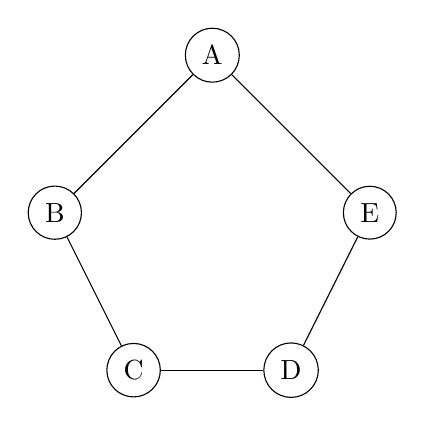
\begin{tikzpicture}
    \node[shape=circle,draw=black] (C) at (1,0) {C};
    \node[shape=circle,draw=black] (B) at (0,2) {B};
    \node[shape=circle,draw=black] (A) at (2,4) {A};
    \node[shape=circle,draw=black] (D) at (3,0) {D};
    \node[shape=circle,draw=black] (E) at (4,2) {E};
    \path [] (A) edge node[left] {} (B);
    \path [] (B) edge node[left] {} (C);
    \path [] (C) edge node[left] {} (D);
    \path [] (D) edge node[left] {} (E);
    \path [] (E) edge node[left] {} (A);
\end{tikzpicture}
\end{align*}

\begin{question}{4} 
	Let $A$ be the adjacency matrix of  $K_n$. If i = j , then $A^{2}[i,j]$\_\_\_\_.  Otherwise, $A^{2}[i,j]$ =\_\_\_\_. 
\end{question}

\begin{itemize}
\item If i = j , then $A^{2}[i,j]$ = (n-1)
\item Otherwise,   $A^{2}[i,j]$ = (n-2)
\end{itemize}


\begin{question}{2}
	Find all metamorphism classes of simple graphs with 5 vertices and 5 edges.
\end{question}


\begin{align*}
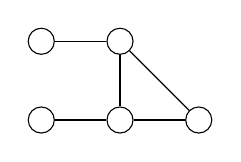
\begin{tikzpicture}
\node[shape=circle,draw=black] (A) at (0,0) {};
\node[shape=circle,draw=black] (B) at (1,0) {};
\node[shape=circle,draw=black] (C) at (0,-1) {};
\node[shape=circle,draw=black] (D) at (1,-1) {};
\node[shape=circle,draw=black] (E) at (2,-1) {};
\path [] (A) edge node[left] {} (B);
\path [] (C) edge node[left] {} (D);
\path [] (B) edge node[left] {} (D);
\path [] (B) edge node[left] {} (E);
\path [] (D) edge node[left] {} (E);
\end{tikzpicture}
\end{align*}



\begin{align*}
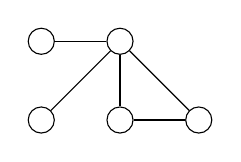
\begin{tikzpicture}
\node[shape=circle,draw=black] (A) at (0,0) {};
\node[shape=circle,draw=black] (B) at (1,0) {};
\node[shape=circle,draw=black] (C) at (0,-1) {};
\node[shape=circle,draw=black] (D) at (1,-1) {};
\node[shape=circle,draw=black] (E) at (2,-1) {};
\path [] (A) edge node[left] {} (B);
\path [] (C) edge node[left] {} (B);
\path [] (B) edge node[left] {} (D);
\path [] (B) edge node[left] {} (E);
\path [] (D) edge node[left] {} (E);
\end{tikzpicture}
\end{align*}

\begin{align*}
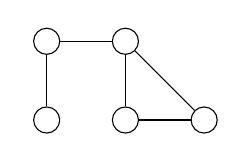
\begin{tikzpicture}
\node[shape=circle,draw=black] (A) at (0,0) {};
\node[shape=circle,draw=black] (B) at (1,0) {};
\node[shape=circle,draw=black] (C) at (0,-1) {};
\node[shape=circle,draw=black] (D) at (1,-1) {};
\node[shape=circle,draw=black] (E) at (2,-1) {};
\path [] (A) edge node[left] {} (B);
\path [] (C) edge node[left] {} (A);
\path [] (B) edge node[left] {} (D);
\path [] (B) edge node[left] {} (E);
\path [] (D) edge node[left] {} (E);
\end{tikzpicture}
\end{align*}


\begin{align*}
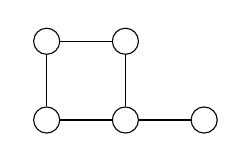
\begin{tikzpicture}
\node[shape=circle,draw=black] (A) at (0,0) {};
\node[shape=circle,draw=black] (B) at (1,0) {};
\node[shape=circle,draw=black] (C) at (0,-1) {};
\node[shape=circle,draw=black] (D) at (1,-1) {};
\node[shape=circle,draw=black] (E) at (2,-1) {};
\path [] (A) edge node[left] {} (B);
\path [] (C) edge node[left] {} (D);
\path [] (B) edge node[left] {} (D);
\path [] (A) edge node[left] {} (C);
\path [] (D) edge node[left] {} (E);
\end{tikzpicture}
\end{align*}

\begin{align*}
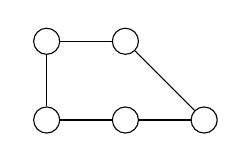
\begin{tikzpicture}
\node[shape=circle,draw=black] (A) at (0,0) {};
\node[shape=circle,draw=black] (B) at (1,0) {};
\node[shape=circle,draw=black] (C) at (0,-1) {};
\node[shape=circle,draw=black] (D) at (1,-1) {};
\node[shape=circle,draw=black] (E) at (2,-1) {};
\path [] (A) edge node[left] {} (B);
\path [] (B) edge node[left] {} (E);
\path [] (D) edge node[left] {} (E);
\path [] (A) edge node[left] {} (C);
\path [] (D) edge node[left] {} (C);
\end{tikzpicture}
\end{align*}



\begin{align*}
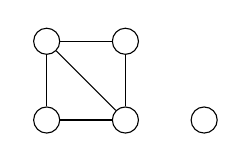
\begin{tikzpicture}
\node[shape=circle,draw=black] (A) at (0,0) {};
\node[shape=circle,draw=black] (B) at (1,0) {};
\node[shape=circle,draw=black] (C) at (0,-1) {};
\node[shape=circle,draw=black] (D) at (1,-1) {};
\node[shape=circle,draw=black] (E) at (2,-1) {};
\path [] (A) edge node[left] {} (B);
\path [] (B) edge node[left] {} (D);
\path [] (D) edge node[left] {} (C);
\path [] (A) edge node[left] {} (C);
\path [] (D) edge node[left] {} (A);
\end{tikzpicture}
\end{align*}

\begin{question}{3}
	Determine which pairs of graphs below are bipartite.
	
	
	\begin{align*}
	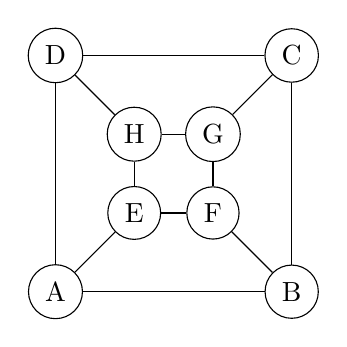
\begin{tikzpicture}
	\node[shape=circle,draw=black] (A) at (0,-3) {A};
	\node[shape=circle,draw=black] (B) at (3,-3) {B};
	\node[shape=circle,draw=black] (C) at (3,0) {C};
	\node[shape=circle,draw=black] (D) at (0,0) {D};
	\node[shape=circle,draw=black] (E) at (1,-2) {E};
	\node[shape=circle,draw=black] (F) at (2,-2) {F};
	\node[shape=circle,draw=black] (G) at (2,-1) {G};
	\node[shape=circle,draw=black] (H) at (1,-1) {H};
	\path [] (D) edge node[left] {} (A);
	\path [] (A) edge node[left] {} (B);
	\path [] (B) edge node[left] {} (C);
	\path [] (C) edge node[left] {} (D);
	\path [] (E) edge node[left] {} (F);
	\path [] (F) edge node[left] {} (G);
	\path [] (G) edge node[left] {} (H);
	\path [] (H) edge node[left] {} (E);
	\path [] (A) edge node[left] {} (E);
	\path [] (B) edge node[left] {} (F);
	\path [] (G) edge node[left] {} (C);
	\path [] (D) edge node[left] {} (H);
	\end{tikzpicture}
	\end{align*}
	
	\begin{align*}
	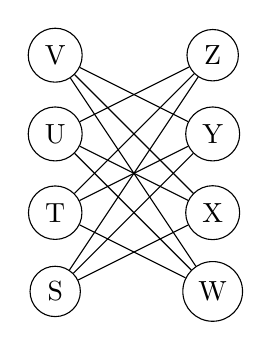
\begin{tikzpicture}
	\node[shape=circle,draw=black] (S) at (0,0) {S};
	\node[shape=circle,draw=black] (T) at (0,1) {T};
	\node[shape=circle,draw=black] (U) at (0,2) {U};
	\node[shape=circle,draw=black] (V) at (0,3) {V};
	\node[shape=circle,draw=black] (W) at (2,0) {W};
	\node[shape=circle,draw=black] (X) at (2,1) {X};
	\node[shape=circle,draw=black] (Y) at (2,2) {Y};
	\node[shape=circle,draw=black] (Z) at (2,3) {Z};
	\path [] (S) edge node[left] {} (Z);
	\path [] (S) edge node[left] {} (Y);
	\path [] (S) edge node[left] {} (X);
	\path [] (T) edge node[left] {} (Z);
	\path [] (T) edge node[left] {} (Y);
	\path [] (T) edge node[left] {} (W);
	\path [] (U) edge node[left] {} (Z);
	\path [] (U) edge node[left] {} (X);
	\path [] (U) edge node[left] {} (W);
	\path [] (V) edge node[left] {} (Y);
	\path [] (V) edge node[left] {} (X);
	\path [] (V) edge node[left] {} (W);
	\end{tikzpicture}
	\end{align*}
	
\end{question}
	
	The first and second graph are isomorphic. The first can be relabeled to look like the second:
		\begin{align*}
	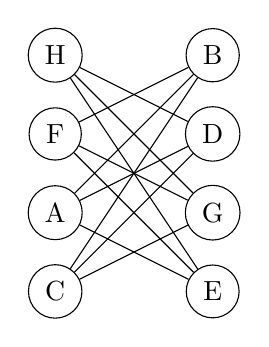
\begin{tikzpicture}
	\node[shape=circle,draw=black] (C) at (0,0) {C};
	\node[shape=circle,draw=black] (A) at (0,1) {A};
	\node[shape=circle,draw=black] (F) at (0,2) {F};
	\node[shape=circle,draw=black] (H) at (0,3) {H};
	\node[shape=circle,draw=black] (E) at (2,0) {E};
	\node[shape=circle,draw=black] (G) at (2,1) {G};
	\node[shape=circle,draw=black] (D) at (2,2) {D};
	\node[shape=circle,draw=black] (B) at (2,3) {B};
	\path [] (D) edge node[left] {} (A);
	\path [] (A) edge node[left] {} (B);
	\path [] (B) edge node[left] {} (C);
	\path [] (C) edge node[left] {} (D);
	\path [] (E) edge node[left] {} (F);
	\path [] (F) edge node[left] {} (G);
	\path [] (G) edge node[left] {} (H);
	\path [] (H) edge node[left] {} (E);
	\path [] (A) edge node[left] {} (E);
	\path [] (B) edge node[left] {} (F);
	\path [] (G) edge node[left] {} (C);
	\path [] (D) edge node[left] {} (H);
	\end{tikzpicture}
	\end{align*}
	
	The third graph is not isomorphic, because it is not a bipartite graph like the first two graphs.	
	
\begin{question}{5}
	Prove or disprove: if $G$ is a disconnected graph, then $\overline{G}$, the complement of $G$, is connected.\\	
	
	i. Let $u$, $v$ be on different components in $G$. Since there is no $uv$ edge in $G$, there must be a $uv$ edge in $\overline{G}$. Thus $u$ $v$ are connected in $\overline{G}$\\
		
	ii. Let $u$, $v$ be on the same component in $G$. Let $w$ be a vertex on a separate component in $G$. There must be a $uw$ edge in $\overline{G}$. There must also be a $vw$ edge in $\overline{G}$. 

	Because there is a $uw$ path, and a $vw$ path, by Lemma 1.2.5 there must also be a $uv$ path. Thus $u$ and $v$ are connected in $\overline{G}$\\

	Because there exists a path between any two vertices in $\overline{G}$ it is a connected graph.
\end{question}

\begin{question}{6}
Determine whether $K_4$ contains the following (give an example or a proof of non-existence);
\end{question}
a) A walk that is not a trail. \\
\begin{align*}
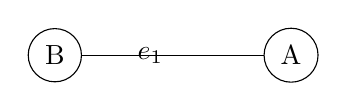
\begin{tikzpicture}
    \node[shape=circle,draw=black] (A) at (3,0) {A};
    \node[shape=circle,draw=black] (B) at (0,0) {B};
    \path [] (A) edge node[left] {$e_1$} (B);
\end{tikzpicture}
\end{align*}

The walk B, $e_1$, A, $e_1$, B is a walk that is not a trail. \\ \\
b) A trail that is not closed and is not a path. \\
\begin{align*}
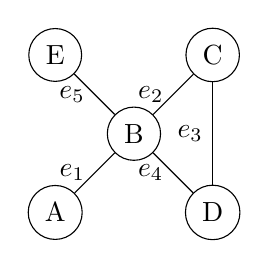
\begin{tikzpicture}
    \node[shape=circle,draw=black] (A) at (0,0) {A};
    \node[shape=circle,draw=black] (B) at (1,1) {B};
    \node[shape=circle,draw=black] (C) at (2,2) {C};
    \node[shape=circle,draw=black] (D) at (2,0) {D};
    \node[shape=circle,draw=black] (E) at (0,2) {E};
    \path [] (A) edge node[left] {$e_1$} (B);
    \path [] (B) edge node[left] {$e_2$} (C);
    \path [] (C) edge node[left] {$e_3$} (D);
    \path [] (D) edge node[left] {$e_4$} (B);
    \path [] (B) edge node[left] {$e_5$} (E);
\end{tikzpicture}
\end{align*}
The walk A, $e_1$, B, $e_2$, C, $e_3$, D, $e_4$, B, $e_5$, E is a trail that is not closed and is not a path, as the vertex B is repeated. \\

c) A closed trail that is not a cycle. \\
\begin{align*}

\begin{tikzpicture}
    \node[shape=circle,draw=black] (A) at (0,0) {A};
\end{tikzpicture}
\end{align*}

The closed trail of A alone is a closed trail that is not a cycle. \\

\begin{question}{7}
A graph is called chordal if it has no induced subgraph isomorphic to $C_{n}$ for any $n \leq 4$. Which of the following 10-vertex graphs are chordal?
\end{question}

\begin{itemize}
\item $K_{10}$ \hspace{3mm}: Yes
\item $K_{5,5}$ \hspace{2mm}: No
\item $K_{1,9}$ \hspace{2mm}: Yes
\item $C_{10}$ \hspace{3mm}: No
\item $P_{10}$ \hspace{3mm}: Yes
\item Peterson Graph: No
\end{itemize}

\begin{align*}
\end{align*}

\begin{question}{8}
a. For each graph $G$ below, find the incidence matrix $M(G)$. (See definition 1.1.17 and Example 1.1.19.)
\begin{center}
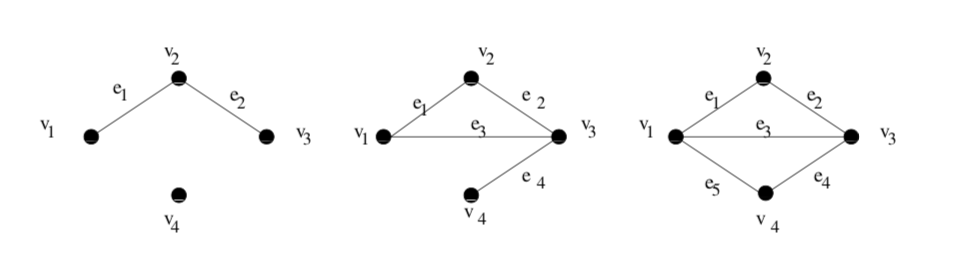
\includegraphics{q8.png}
\end{center}
\end{question}

\begin{tabular}{|c|c|c|} 
\multicolumn{3}{c}{Far Left}  \\ \hline
 & e$_1$ & e$_2$ \\ \hline
v$_1$ & 1 & 0 \\ \hline
v$_2$ & 1 & 1 \\ \hline
v$_3$ & 0 & 1 \\ \hline
v$_4$ & 0 & 0 \\ \hline
\end{tabular}

\begin{tabular}{|c|c|c|c|c|} 
\multicolumn{5}{c}{Middle}  \\ \hline
 & e$_1$ & e$_2$ & e$_3$ & e$_4$ \\ \hline
v$_1$ & 1 & 0 & 1 & 0 \\ \hline
v$_2$ & 1 & 1 & 0 & 0 \\ \hline
v$_3$ & 0 & 1 & 1 & 1 \\ \hline
v$_4$ & 0 & 0 & 0 & 1\\ \hline
\end{tabular}

\begin{tabular}{|c|c|c|c|c|c|} 
\multicolumn{6}{c}{Far Right}  \\ \hline
 & e$_1$ & e$_2$ & e$_3$ & e$_4$ & e$_5$\\ \hline
v$_1$ & 1 & 0 & 1 & 0 & 1 \\ \hline
v$_2$ & 1 & 1 & 0 & 0 & 0 \\ \hline
v$_3$ & 0 & 1 & 1 & 1 & 0 \\ \hline
v$_4$ & 0 & 0 & 0 & 1 & 1 \\ \hline
\end{tabular}

b. Recall that the transpose of a $ p \times q$ matrix $M$ is the $ q \times p $ matrix $M^{T}$ with $ M^{T}[i,j] = M[j,i]$. For each graph $G$ above in (a), find the matrix product $M(G) \cdot (M(G))^{T}$. \\ \\

\begin{tabular}{|c|c|c|c|} 
\multicolumn{4}{c}{Far Left}  \\ \hline
1 & 1 & 0 & 0 \\ \hline
1 & 2 & 1 & 0 \\ \hline
0 & 1 & 1 & 0 \\ \hline
0 & 0 & 0 & 0\\ \hline
\end{tabular}

\begin{tabular}{|c|c|c|c|} 
\multicolumn{4}{c}{Middle}  \\ \hline
2 & 1 & 1 & 0 \\ \hline
1 & 2 & 1 & 0 \\ \hline
1 & 1 & 3 & 1 \\ \hline
0 & 0 & 1 & 1\\ \hline
\end{tabular}

\begin{tabular}{|c|c|c|c|} 
\multicolumn{4}{c}{Far Right}  \\ \hline
3 & 1 & 1 & 1 \\ \hline
1 & 2 & 1 & 0 \\ \hline
1 & 1 & 3 & 1 \\ \hline
1 & 0 & 1 & 2\\ \hline
\end{tabular}




% --------------------------------------------------------------
%     You don't have to mess with anything below this line.
% --------------------------------------------------------------

\end{document}
